\let\negmedspace\undefined
\let\negthickspace\undefined
\documentclass[journal]{IEEEtran}
\usepackage[a5paper, margin=10mm, onecolumn]{geometry}
%\usepackage{lmodern} % Ensure lmodern is loaded for pdflatex
\usepackage{tfrupee} % Include tfrupee package

\setlength{\headheight}{1cm} % Set the height of the header box
\setlength{\headsep}{0mm}     % Set the distance between the header box and the top of the text

\usepackage{gvv-book}
\usepackage{gvv}
\usepackage{cite}
\usepackage{amsmath,amssymb,amsfonts,amsthm}
\usepackage{algorithmic}
\usepackage{graphicx}
\usepackage{textcomp}
\usepackage{xcolor}
\usepackage{txfonts}
\usepackage{listings}
\usepackage{enumitem}
\usepackage{mathtools}
\usepackage{gensymb}
\usepackage{comment}
\usepackage[breaklinks=true]{hyperref}
\usepackage{tkz-euclide} 
\usepackage{listings}
% \usepackage{gvv}                                        
\def\inputGnumericTable{}                                 
\usepackage[latin1]{inputenc}                                
\usepackage{color}                                            
\usepackage{array}                                            
\usepackage{longtable}                                       
\usepackage{calc}  
\usepackage{amsmath,amssymb}

\usepackage{multicol}                                         
\usepackage{hhline}                                           
\usepackage{ifthen}                                           
\usepackage{lscape}
\begin{document}

\bibliographystyle{IEEEtran}

\title{
%	\logo{
GATE

\large{EE1030}

2008
%	}
}
\author{Homa Harshitha Vuddanti

(EE24BTECH11062)
}	

\maketitle

\bigskip

\renewcommand{\thefigure}{\theenumi}
\renewcommand{\thetable}{\theenumi}
QUESTIONS- 1 to 17\\
\begin{enumerate}
   
\item In the Taylor series expansion of $e^x$ about $x=2$, the coefficient of $\brak{x-2}^4$ is
\begin{multicols}{4}
    a) $\frac{1}{4!}$\\
    b) $\frac{2^4}{4!}$\\
    c) $\frac{e^2}{4!}$\\
    d)  $\frac{e^4}{4!}$
\end{multicols}
 \item Given that $\ddot{x}+3x=0$, and $x\brak{0}=1,\dot{x}\brak{0}=0,
$ what is $x\brak{1}?$

 \begin{multicols}{4}
     a) -0.99\\
     b) -0.16\\
     c) 0.16\\
     d) 0.99
 \end{multicols}
 
 \item The value of $\lim_{x \to 8} \frac{x^{1/3}-2}{\brak{x-8}}$ is
 \begin{multicols}{4}
    a) $\frac{1}{16}$\\
    b) $\frac{1}{12}$\\
    c)  $\frac{1}{8}$\\
    d)  $\frac{1}{4}$
 \end{multicols}
 
\item A coin is tossed 4 times. What is the probability of getting heads exactly 3 times?
\begin{multicols}{4}
    a) $\frac{1}{4}$\\
    b) $\frac{3}{8}$\\
    c)  $\frac{1}{2}$\\
    d)  $\frac{3}{4}$
\end{multicols}

\item The matrix $\begin{bmatrix}1 && 2 && 4 \\ 3 && 0 && 6\\1 && 1 && p\end{bmatrix}$ has one eigenvalue equal to 3. The sum of the other two eigenvalues is
\begin{multicols}{4}
    a) $p$\\
    b) $p-1$\\
    c) $p-2$\\
    d) $p-3$
\end{multicols}
\item The divergence of the vector field $\brak{x-y}\hat{i}
+\brak{y-x}\hat{j}+\brak{x+y+z}\hat{k}
$ is
\begin{multicols}{4}
    a) 0\\
    b) 1\\
    c) 2\\
    d) 3
\end{multicols}

\item The transverse shear stress acting in a beam of rectangular cross-section, subjected to a transverse shear load, is
\begin{enumerate}
    \item variable with maximum at bottom of the beam
    \item variable with maximum at top of the beam
    \item uniform
    \item variable with maximum on the neutral axis
\end{enumerate}
\item A rod of length $L$ and diameter $D$ is subjected to a tensile load $P$. Which of the following is sufficient to calculate the resulting change in diameter?
\begin{enumerate}
    \item Young's modulus
    \item Shear modulus
    \item Poisson's ratio
    \item Both Young's modulus and shear modulus
\end{enumerate}

\item A straight rod of length $L\brak{t}$, hinged at one end and freely extensible at the other end, rotates through an angle $\theta\brak{t}$ about the hinge. The time $t$, $L\brak{t}=1m$ , $L\brak{t}= 1 m/s$, $\theta\brak{t}=\frac{\pi}{4}$rad and $\theta\brak{t}= 1$rad/s. The magnitude of the velocity at the other end of the rod is
\begin{multicols}{4}
     a) 1 m/s\\
     b) $\sqrt{2}$ m/s\\
     c) $\sqrt{3}$ m/s\\
     d) 2 m/s
 \end{multicols}

\item A cantilever type gate hinged at $Q$ is shown in the figure. P and R are the centres of gravity of the cantilever part and the counterweight respectively. The mass of the cantilever part is 75 kg. The mass of the counterweight, for static balance, is

\begin{center}
   \scalebox{0.75}{
\begin{tikzpicture}
    % Draw the counterweight rectangle
    \draw[thick] (-1, -1) rectangle (0, 1);

    % Draw the cantilever part (triangle pointing to the right)
    \draw[thick] (5,0) -- (0,0.5) -- (0,-0.5) -- cycle;

    % Mark and label points R, Q, and P
    \filldraw (-0.5,0) circle (2pt) node[above left] {R};
    \filldraw (0.5,0) circle (2pt) node[above right] {Q};
    \filldraw (2.5,0) circle (2pt) node[above right] {P};

    % Add distance labels with arrows
    \draw[<->] (-0.5, -1.5) -- (0.5, -1.5) node[midway, below] {0.5 m};
    \draw[<->] (0.5, -1.5) -- (2.5, -1.5) node[midway, below] {2.0 m};

    % Draw the support line at Q and vertical distance indicators
    \draw[thick] (0, -1.25) -- (0, 1.25);

\end{tikzpicture}
}
\end{center}

\begin{multicols}{4}
     a) 75 kg\\
     b) 150 kg\\
     c) 225 kg\\
     d) 300 kg
 \end{multicols}

\item A planar mechanism has 8 links and 10 rotary joints. The number of degrees of freedom of the mechanism, using Gruebler's criterion, is
\begin{multicols}{4}
     a) 0\\
     b) 1\\
     c) 2\\
     d) 3
 \end{multicols}

\item An axial residual compressive stress due to a manufacturing process is present on the outer surface of a rotating shaft subjected to bending. Under a given bending load, the fatigue life of the shaft in the presence of the residual compressive stress is
\begin{enumerate}
    \item decreased
    \item increased or decreased, depending on the external bending load
    \item neither increased nor decreased
    \item increased
\end{enumerate}

\item 2 moles of oxygen are mixed adiabatically with another 2 moles of oxygen in a mixing chamber, so that the final total pressure and temperature of the mixture become same as those of individual constituents at their initial states. The universal gas constant is given as $R$. The change in entropy due to mixing, per mole of oxygen, is given by
\begin{multicols}{4}
     a) $-R\ln{2}$\\
     b) 0\\
     c) $R\ln{2}$\\
     d) $R \ln{4}$
 \end{multicols}
 \item For flow of fluid over a heated plate, the following fluid properties are known:
 viscosity = 0.001 Pa.s ; specific heat at constant pressure = 1kJ/kg.K ; thermal conductivity = 1 W/m.K.
 The hydrodynamic boundary layer thickness at a specific location on the plate is 1 mm. The thermal boundary layer thickness at the same location is
\begin{multicols}{4}
     a) 0.001 mm\\
     b) 0.01 mm\\
     c) 1 mm\\
     d) 1000 mm
 \end{multicols}
\item For the continuity equation given by $\overrightarrow{V}\cdot \overrightarrow{V}=0$ to be valid, where $\overrightarrow{V}
$ is the velocity vector, which one of the following is a necessary condition?
\begin{enumerate}
    \item steady flow
    \item irrotational flow
    \item inviscid flow
    \item incompressible flow
\end{enumerate}
\item Which one of the following is NOT a necessary assumption for the air-standard Otto  cycle?
\begin{enumerate}
    \item All processes are both internally as well as externally reversible.
    \item Intake and exhaust processes are constant volume heat rejection processes.
    \item The combustion process is a constant volume heat addition process
    \item The working fluid is an ideal gas with constant specific heats.
\end{enumerate}
\item In an M/M/I queuing system, the number of arrivals in an interval of length $T$ is a Poisson random variable (i.e. the probability of there being $n$ arrivals in an interval of length $T$ is $\frac{e^{-\lambda T}\brak{\lambda T}^n}{n!}$). The probability density function $f\brak{t}$ of the inter-arrival time is given by
\begin{multicols}{4}
     a) $-R\ln{2}$\\
     b) 0\\
     c) $R\ln{2}$\\
     d) $R \ln{4}$
 \end{multicols}
\end{enumerate}
\end{document}


